
			\level{4}[ViewModel]{Chuck::ViewModel}
			

		\IfFileExists{DefinizioneDiProdotto/Pics/Classi/Chuck--ViewModel.pdf}{
			\begin{figure}[H]
				\centering
				\includegraphics[scale=0.5]{DefinizioneDiProdotto/Pics/Classi/Chuck--ViewModel}
				\caption{Chuck::ViewModel}
			\end{figure}
		}
	

			\begin{itemize}
			\item \textbf{Nome:} ViewModel
			\item \textbf{Tipo:} package
			
			\item \textbf{Descrizione:} ViewModel è il package che fa da tramite tra la View e il Model. Le sue classi si occupano di richiamare le funzionalità delle librerie grafiche che permettono alla View di visualizzare i grafici. Inoltre hanno lo scopo di ricevere gli input provenienti dalla View ed effettuarne la gestione. L’input consiste in un sottoinsieme di dataset scelti dall’utente che sta visualizzando la pagina web. Il ViewModel deve far sì che vengano visualizzati solo questi dataset, in modo da permettere all’utente di applicare un filtro sulle serie.
			\end{itemize}

			
			\level{5}[BarChartViewModel]{Chuck::ViewModel::BarChartViewModel}
			

		\IfFileExists{DefinizioneDiProdotto/Pics/Classi/Chuck--ViewModel--BarChartViewModel.pdf}{
			\begin{figure}[H]
				\centering
				\includegraphics[scale=0.5]{DefinizioneDiProdotto/Pics/Classi/Chuck--ViewModel--BarChartViewModel}
				\caption{Chuck::ViewModel::BarChartViewModel}
			\end{figure}
		}
	
			
			\begin{itemize}
			\item \textbf{Nome:} BarChartViewModel
			\item \textbf{Tipo:} classe
			
		\item \textbf{Estende:}
		ChartViewModel
		\item \textbf{Astratta:}
		no
			\item \textbf{Visibilità:} public
			\item \textbf{Descrizione:} BarChartViewModel specializza ChartVewModel e costituice una view per i grafici di tipo BarChart. Essa utilizza la libreria Chart.js per la rappresentazione grafica del bar chart.
			\item \textbf{Attributi:}
				\begin{itemize}
				\setlength{\itemsep}{5pt}
				
					\item[\ding{111}] {--lib : GoogleChart} \\ [1mm] Questo attributo è un riferimento alla libreria utilizzata per renderizzare il grafico.
				\end{itemize}
		
			\item \textbf{Metodi:}
				\begin{itemize}
				\setlength{\itemsep}{5pt}
				
					\item[\ding{111}] {{\#init() : void}} \\ [1mm] Tale metodo permette di inizializzare la view e visualizzare il BarChart secondo i dati memorizzati.
					\item[\ding{111}] {{\#render(newValue : ChartImpl, oldValue : ChartImpl) : void}} \\ [1mm] Tale metodo permette di aggiornare la visualizzazione del BarChart secondo i nuovi dati. I parametri newValue e oldValue rappresentano rispettivamente i nuovi valori e quelli vecchi.
				\end{itemize}
		
			\end{itemize}

			
			\level{5}[ChartViewModel]{Chuck::ViewModel::ChartViewModel}
			

		\IfFileExists{DefinizioneDiProdotto/Pics/Classi/Chuck--ViewModel--ChartViewModel.pdf}{
			\begin{figure}[H]
				\centering
				\includegraphics[scale=0.5]{DefinizioneDiProdotto/Pics/Classi/Chuck--ViewModel--ChartViewModel}
				\caption{Chuck::ViewModel::ChartViewModel}
			\end{figure}
		}
	
			
			\begin{itemize}
			\item \textbf{Nome:} ChartViewModel
			\item \textbf{Tipo:} classe
			
		\item \textbf{Astratta:}
		si
			\item \textbf{Visibilità:} package
			\item \textbf{Descrizione:} ChartViewModel è una classe astratta che rappresenta una view generica.
			\item \textbf{Attributi:}
				\begin{itemize}
				\setlength{\itemsep}{5pt}
				
					\item[\ding{111}] {\#chart : ChartImpl}
				\end{itemize}
		
			\item \textbf{Metodi:}
				\begin{itemize}
				\setlength{\itemsep}{5pt}
				
					\item[\ding{111}] \textit{{\#init() : void}} \\ [1mm] Tale metodo permette di inizializzare la view e visualizzare il grafico secondo i dati memorizzati.
					\item[\ding{111}] \textit{{\#render(newValue : ChartImpl, oldValue : ChartImpl) : void}} \\ [1mm] Tale è astratto ed identifica un metodo che permette di aggiornare la visualizzazione del grafico secondo i nuovi dati. I parametri newValue e oldValue rappresentano rispettivamente i nuovi valori e quelli vecchi.
				\end{itemize}
		
			\end{itemize}

			
			\level{5}[LineChartViewModel]{Chuck::ViewModel::LineChartViewModel}
			

		\IfFileExists{DefinizioneDiProdotto/Pics/Classi/Chuck--ViewModel--LineChartViewModel.pdf}{
			\begin{figure}[H]
				\centering
				\includegraphics[scale=0.5]{DefinizioneDiProdotto/Pics/Classi/Chuck--ViewModel--LineChartViewModel}
				\caption{Chuck::ViewModel::LineChartViewModel}
			\end{figure}
		}
	
			
			\begin{itemize}
			\item \textbf{Nome:} LineChartViewModel
			\item \textbf{Tipo:} classe
			
		\item \textbf{Estende:}
		ChartViewModel
		\item \textbf{Astratta:}
		no
			\item \textbf{Visibilità:} public
			\item \textbf{Descrizione:} LineChartViewModel specializza ChartViewModel e costituice una view per i grafici di tipo LineChart. Essa utilizza la libreria Chart.js per la rappresentazione grafica del line chart.
			\item \textbf{Attributi:}
				\begin{itemize}
				\setlength{\itemsep}{5pt}
				
					\item[\ding{111}] {--lib : GoogleChart} \\ [1mm] Questo attributo è un riferimento alla libreria utilizzata per renderizzare il grafico.
				\end{itemize}
		
			\item \textbf{Metodi:}
				\begin{itemize}
				\setlength{\itemsep}{5pt}
				
					\item[\ding{111}] {{\#init() : void}} \\ [1mm] Tale metodo permette di inizializzare la view e visualizzare il LineChart secondo i dati memorizzati.
					\item[\ding{111}] {{\#render(newValue : ChartImpl, oldValue : ChartImpl) : void}} \\ [1mm] Tale metodo permette di aggiornare la visualizzazione del LineChart secondo i nuovi dati. I parametri newValue e oldValue rappresentano rispettivamente i nuovi valori e quelli vecchi.
				\end{itemize}
		
			\end{itemize}

			
			\level{5}[MapChartViewModel]{Chuck::ViewModel::MapChartViewModel}
			

		\IfFileExists{DefinizioneDiProdotto/Pics/Classi/Chuck--ViewModel--MapChartViewModel.pdf}{
			\begin{figure}[H]
				\centering
				\includegraphics[scale=0.5]{DefinizioneDiProdotto/Pics/Classi/Chuck--ViewModel--MapChartViewModel}
				\caption{Chuck::ViewModel::MapChartViewModel}
			\end{figure}
		}
	
			
			\begin{itemize}
			\item \textbf{Nome:} MapChartViewModel
			\item \textbf{Tipo:} classe
			
		\item \textbf{Estende:}
		ChartViewModel
		\item \textbf{Astratta:}
		no
			\item \textbf{Visibilità:} public
			\item \textbf{Descrizione:} MapChartViewModel specializza ChartViewModel e costituice una view per i grafici di tipo MapChart. Essa utilizza la libreria OpenStreetMap per la rappresentazione grafica del map chart.
			\item \textbf{Attributi:}
				\begin{itemize}
				\setlength{\itemsep}{5pt}
				
					\item[\ding{111}] {--lib : OpenStreetMaps} \\ [1mm] Questo attributo è un riferimento alla libreria utilizzata per renderizzare il grafico.
				\end{itemize}
		
			\item \textbf{Metodi:}
				\begin{itemize}
				\setlength{\itemsep}{5pt}
				
					\item[\ding{111}] {{\#init() : void}} \\ [1mm] Tale metodo permette di inizializzare la view e visualizzare il MapChart secondo i dati memorizzati.
					\item[\ding{111}] {{\#render(newValue : ChartImpl, oldValue : ChartImpl) : void}} \\ [1mm] Tale metodo permette di aggiornare la visualizzazione del MapChart secondo i nuovi dati. I parametri newValue e oldValue rappresentano rispettivamente i nuovi valori e quelli vecchi.
				\end{itemize}
		
			\end{itemize}

			
			\level{5}[TableViewModel]{Chuck::ViewModel::TableViewModel}
			

		\IfFileExists{DefinizioneDiProdotto/Pics/Classi/Chuck--ViewModel--TableViewModel.pdf}{
			\begin{figure}[H]
				\centering
				\includegraphics[scale=0.5]{DefinizioneDiProdotto/Pics/Classi/Chuck--ViewModel--TableViewModel}
				\caption{Chuck::ViewModel::TableViewModel}
			\end{figure}
		}
	
			
			\begin{itemize}
			\item \textbf{Nome:} TableViewModel
			\item \textbf{Tipo:} classe
			
		\item \textbf{Estende:}
		ChartViewModel
		\item \textbf{Astratta:}
		no
			\item \textbf{Visibilità:} public
			\item \textbf{Descrizione:} TableViewModel specializza ChartViewModel e costituice una view per i grafici di tipo Table. Essa utilizza la libreria DataTables per la rappresentazione grafica della table.
			\item \textbf{Attributi:}
				\begin{itemize}
				\setlength{\itemsep}{5pt}
				
					\item[\ding{111}] {--lib : DataTables}
				\end{itemize}
		
			\item \textbf{Metodi:}
				\begin{itemize}
				\setlength{\itemsep}{5pt}
				
					\item[\ding{111}] {{\#init() : void}} \\ [1mm] Tale metodo permette di inizializzare la view e visualizzare la Table secondo i dati memorizzati.
					\item[\ding{111}] {{\#render(newValue : ChartImpl, oldValue : ChartImpl) : void}} \\ [1mm] Tale metodo permette di aggiornare la visualizzazione della Table secondo i nuovi dati. I parametri newValue e oldValue rappresentano rispettivamente i nuovi valori e quelli vecchi.
				\end{itemize}
		
			\end{itemize}

			
			\level{4}[Model]{Chuck::Model}
			

		\IfFileExists{DefinizioneDiProdotto/Pics/Classi/Chuck--Model.pdf}{
			\begin{figure}[H]
				\centering
				\includegraphics[scale=0.5]{DefinizioneDiProdotto/Pics/Classi/Chuck--Model}
				\caption{Chuck::Model}
			\end{figure}
		}
	

			\begin{itemize}
			\item \textbf{Nome:} Model
			\item \textbf{Tipo:} package
			
			\item \textbf{Descrizione:} Model è il package che contiene il modello dei dati e i servizi di business logic. Infatti in esso sono presenti due sottopackage
			\end{itemize}

			
			\level{4}[NorrisChart]{Chuck::Model::NorrisChart}
			

		\IfFileExists{DefinizioneDiProdotto/Pics/Classi/Chuck--Model--NorrisChart.pdf}{
			\begin{figure}[H]
				\centering
				\includegraphics[scale=0.5]{DefinizioneDiProdotto/Pics/Classi/Chuck--Model--NorrisChart}
				\caption{Chuck::Model::NorrisChart}
			\end{figure}
		}
	

			\begin{itemize}
			\item \textbf{Nome:} NorrisChart
			\item \textbf{Tipo:} package
			
			\item \textbf{Descrizione:} NorrisChart contiene i dati riguardanti i grafici, assieme alle relative impostazioni. In particolare sono presenti i modelli di tutte le tipologie di chart implementati da Norris, ovvero Bar Chart, Line Chart, Map Chart e Table. Per ciascuna tipologia di grafico sono forniti i metodi per inserire i dati e configurare alcune impostazioni. Fornisce inoltre dei metodi per ottenere i valori di queste ultime, in modo da poterle riutilizzare per un altro grafico. Infine, per ogni grafico sono disponibili le stesse modalità di aggiornamento fornite da Norris.
			\end{itemize}

			
			\level{5}[BarChartImpl]{Chuck::Model::NorrisChart::BarChartImpl}
			

		\IfFileExists{DefinizioneDiProdotto/Pics/Classi/Chuck--Model--NorrisChart--BarChartImpl.pdf}{
			\begin{figure}[H]
				\centering
				\includegraphics[scale=0.5]{DefinizioneDiProdotto/Pics/Classi/Chuck--Model--NorrisChart--BarChartImpl}
				\caption{Chuck::Model::NorrisChart::BarChartImpl}
			\end{figure}
		}
	
			
			\begin{itemize}
			\item \textbf{Nome:} BarChartImpl
			\item \textbf{Tipo:} classe
			
		\item \textbf{Estende:}
		ChartImpl
		\item \textbf{Astratta:}
		no
			\item \textbf{Visibilità:} package
			\item \textbf{Descrizione:} Questa classe rappresenta un grafico di tipo bar chart. Essa contiene al suo interno i dati (BarChartDataObject) e le impostazioni (BarChartSettingsObject) relativi al grafico. Inoltre contiene la classe BarChartInPlaceUpdater, la quale implementa l'aggiornamento di tipo in place per il grafico in questione. Un'istanza della classe BarChartImpl viene creata dalla classe factory BarChartFactory.

			\item \textbf{Metodi:}
				\begin{itemize}
				\setlength{\itemsep}{5pt}
				
					\item[\ding{111}] {{--BarChartImpl(id : String)}} \\ [1mm] Questo metodo è il costruttore della classe.
				\end{itemize}
		
			\end{itemize}

			
			\level{5}[BarChartFactory]{Chuck::Model::NorrisChart::BarChartImpl::BarChartFactory}
			

		\IfFileExists{DefinizioneDiProdotto/Pics/Classi/Chuck--Model--NorrisChart--BarChartImpl--BarChartFactory.pdf}{
			\begin{figure}[H]
				\centering
				\includegraphics[scale=0.5]{DefinizioneDiProdotto/Pics/Classi/Chuck--Model--NorrisChart--BarChartImpl--BarChartFactory}
				\caption{Chuck::Model::NorrisChart::BarChartImpl::BarChartFactory}
			\end{figure}
		}
	
			
			\begin{itemize}
			\item \textbf{Nome:} BarChartFactory
			\item \textbf{Tipo:} classe
			
		\item \textbf{Astratta:}
		no
			\item \textbf{Visibilità:} private
			\item \textbf{Descrizione:} Questa classe si occupa della creazione di un grafico di tipo BarChartImpl. Tale classe dispone di un blocco di inizializzazione statica che registra la sua istanza nel HashMap factories della classe ChartImpl non appena tale classe viene caricata.
			\item \textbf{Attributi:}
				\begin{itemize}
				\setlength{\itemsep}{5pt}
				
					\item[\ding{111}] \underline{--instance : BarChartFactory} \\ [1mm] Questo attributo è il riferimento all'unica istanza della classe.
				\end{itemize}
		
			\item \textbf{Metodi:}
				\begin{itemize}
				\setlength{\itemsep}{5pt}
				
					\item[\ding{111}] {\underline{+getInstance() : BarChartFactory}} \\ [1mm] Questo metodo permette di ottenere l'unica istanza esistente della classe.
					\item[\ding{111}] {{--BarChartFactory()}} \\ [1mm] Questo metodo è il costruttore della classe. Esso è privato perchè non si vuole permettere a nessuno di poter creare un’istanza se non utilizzando il metodo getInstance().
					\item[\ding{111}] {{+createChart(id : String) : ChartImpl}} \\ [1mm] Tale metodo ha il compito di creare la relativa specializzazione di ChartImpl. Esso può accedere al suo costruttore perchè questa classe factory è interna alla relativa classe BarChartImpl.
				\end{itemize}
		
			\end{itemize}

			
			\level{5}[BarChartInPlaceUpdater]{Chuck::Model::NorrisChart::BarChartInPlaceUpdater}
			

		\IfFileExists{DefinizioneDiProdotto/Pics/Classi/Chuck--Model--NorrisChart--BarChartInPlaceUpdater.pdf}{
			\begin{figure}[H]
				\centering
				\includegraphics[scale=0.5]{DefinizioneDiProdotto/Pics/Classi/Chuck--Model--NorrisChart--BarChartInPlaceUpdater}
				\caption{Chuck::Model::NorrisChart::BarChartInPlaceUpdater}
			\end{figure}
		}
	
			
			\begin{itemize}
			\item \textbf{Nome:} BarChartInPlaceUpdater
			\item \textbf{Tipo:} classe
			
		\item \textbf{Astratta:}
		no
			\item \textbf{Visibilità:} package
			\item \textbf{Descrizione:} Questa classe si occupa di definire il metodo di aggiornamento in place per un grafico di tipo bar chart. Essendo una classe interna di BarChartImpl, ha acceso ai campi dati privati di questa classe. In particolare può accedere al DataObject contenuto in BarChartImpl e modificarne i valori.
			\item \textbf{Attributi:}
				\begin{itemize}
				\setlength{\itemsep}{5pt}
				
					\item[\ding{111}] \underline{--instance : BarChartInPlaceUpdater} \\ [1mm] Questo attributo è il riferimento all'unica istanza della classe.
				\end{itemize}
		
			\item \textbf{Metodi:}
				\begin{itemize}
				\setlength{\itemsep}{5pt}
				
					\item[\ding{111}] {\underline{+getInstance() : BarChartInPlaceUpdater}} \\ [1mm] Questo metodo permette di ottenere l'unica istanza esistente della classe.
					\item[\ding{111}] {{--BarChartInPlaceUpdater()}} \\ [1mm] Questo metodo è il costruttore della classe.
					\item[\ding{111}] {{+update(chart : ChartImpl, updateData : ChartUpdate) : void}} \\ [1mm] Questo metodo permette di aggiornare il chart passato come primo parametro utilizzando i dati passati come secondo parametro.
				\end{itemize}
		
			\end{itemize}

			
			\level{5}[ChartImpl]{Chuck::Model::NorrisChart::ChartImpl}
			

		\IfFileExists{DefinizioneDiProdotto/Pics/Classi/Chuck--Model--NorrisChart--ChartImpl.pdf}{
			\begin{figure}[H]
				\centering
				\includegraphics[scale=0.5]{DefinizioneDiProdotto/Pics/Classi/Chuck--Model--NorrisChart--ChartImpl}
				\caption{Chuck::Model::NorrisChart::ChartImpl}
			\end{figure}
		}
	
			
			\begin{itemize}
			\item \textbf{Nome:} ChartImpl
			\item \textbf{Tipo:} classe
			
		\item \textbf{Astratta:}
		si
			\item \textbf{Visibilità:} public
			\item \textbf{Descrizione:} Questa classe rappresenta un grafico generico e per questo motivo è una classe astratta. Essa contiene al suo interno i dati (ChartData) e le impostazioni (ChartSettings) relativi al grafico. Inoltre contiene l'interfaccia ChartFactory. Sono inoltre presenti due hashmap: la prima si occupa della corrispondenza tra le tipologie di grafico e le rispettive classi factory, la seconda invece si occupa della corrispondenza tra le varie tipologie di aggiornamento e la classe che implementa tale aggiornamento per un tipo specifico di grafico. ChartImpl ha una dipendenza verso l'interfaccia ChartUpdate, in quanto deve conoscere il tipo del pacchetto degli aggiornamenti.
			\item \textbf{Attributi:}
				\begin{itemize}
				\setlength{\itemsep}{5pt}
				
					\item[\ding{111}] \underline{--factories : Map<String,ChartFactory>} \\ [1mm] Questo attributo contiene le dipendenze necessarie per istanziare nuovi grafici.
					\item[\ding{111}] \underline{--updaters : Map<String,ChartUpdater>} \\ [1mm] Questo attributo contiene le dipendenze necessarie per aggiornare i grafici.
					\item[\ding{111}] {--id : String} \\ [1mm] Questo attributo consiste nell'id del grafico.
					\item[\ding{111}] {--type : String} \\ [1mm] Questo attributo consiste nel tipo del grafico.
					\item[\ding{111}] {--data : ChartData} \\ [1mm] Questo attributo contiene i dati rappresentati dal grafico.
					\item[\ding{111}] {--settings : ChartSettings} \\ [1mm] Questo attributo contiene le impostazioni del grafico.
				\end{itemize}
		
			\item \textbf{Metodi:}
				\begin{itemize}
				\setlength{\itemsep}{5pt}
				
					\item[\ding{111}] {\underline{\#registerFactory(chartType : String, factory : ChartFactory) : void}} \\ [1mm] Tale metodo serve per registrare una certa factory al relativo chart nell’hashmap della classe (factories). Tale metodo viene chiamato dalle classi factory interne ai vari ChartImpl con lo scopo di registrarsi come creatori di chart e poter quindi esser utilizzate per tale scopo.
					\item[\ding{111}] {\underline{\#registerUpdater(updateType : String, updater : ChartUpdater) : void}} \\ [1mm] Tale metodo serve per registrare un certo updater al relativo tipo di update nell’HashMap della classe (updaters). Tale metodo viene invocato dalle classi Updater al loro caricamento per aggiungersi come updater.
					\item[\ding{111}] {\underline{+createChart(chartType : String, chartId : String) : ChartImpl}} \\ [1mm] Tale metodo non fa altro che creare il chart associato al parametro type e ritornare l’interfaccia ChartModel di tale istanza creata. Esso non fa altro che invocare il metodo chreateChart dela classe factory pesente nell’HashMap factories con la chiave eguale al parametro type e ne ritornerà tale oggetto creato.
					\item[\ding{111}] {{\#ChartImpl(chartType : String, chartId : String)}} \\ [1mm] Questo metodo è il costruttore della classe. Esso è accessibile solamente alle sottoclassi nella creazione del sottoggetto.
					\item[\ding{111}] {{+getId() : String}} \\ [1mm] Questo metodo permette di ottenere l'id del grafico.
					\item[\ding{111}] {{+getType() : String}} \\ [1mm] Questo metodo permette di ottenere il tipo del grafico.
					\item[\ding{111}] {{+setData(data : ChartData) : void}} \\ [1mm] Questo metodo permette di impostare i dati del grafico.
					\item[\ding{111}] {{+getData() : ChartData}} \\ [1mm] Questo metodo permette di ottenere i dati del grafico.
					\item[\ding{111}] {{+setSettings(settings : ChartSettings) : void}} \\ [1mm] Questo metodo permette di impostare le opzioni del grafico.
					\item[\ding{111}] {{+getSettings() : ChartSettings}} \\ [1mm] Questo metodo permette di ottenere le opzioni del grafico.
					\item[\ding{111}] {{+update(updateType : String, updateData : ChartUpdate) : void}} \\ [1mm] Tale metodo ha il compito di aggiornare i chart utilizzando la tipologia di aggiornamento presente in updateType e il pacchetto di aggiornamento updateData. Esso non fa altro che invocare il metodo update dell’updater pesente nell’hash map updaters con la chiave eguale al parametro updateType e passargli come parametro il parametro ricevuto updateData ed i dati del chart che verranno modificati per riferimento.
				\end{itemize}
		
			\end{itemize}

			
			\level{5}[LineChartImpl]{Chuck::Model::NorrisChart::LineChartImpl}
			

		\IfFileExists{DefinizioneDiProdotto/Pics/Classi/Chuck--Model--NorrisChart--LineChartImpl.pdf}{
			\begin{figure}[H]
				\centering
				\includegraphics[scale=0.5]{DefinizioneDiProdotto/Pics/Classi/Chuck--Model--NorrisChart--LineChartImpl}
				\caption{Chuck::Model::NorrisChart::LineChartImpl}
			\end{figure}
		}
	
			
			\begin{itemize}
			\item \textbf{Nome:} LineChartImpl
			\item \textbf{Tipo:} classe
			
		\item \textbf{Estende:}
		ChartImpl
		\item \textbf{Astratta:}
		no
			\item \textbf{Visibilità:} package
			\item \textbf{Descrizione:} Questa classe rappresenta un grafico di tipo line chart. Essa contiene al suo interno i dati (LineChartDataObject) e le impostazioni (LineChartSettingsObject) relativi al grafico. Inoltre contiene le classi LineChartInPlaceUpdater e LineChartStreamUpdater, le quali implementano rispettivamente l'aggiornamento di tipo in place e stream per il grafico in questione. Un'istanza della classe LineChartImpl viene creata dalla classe factory LineChartFactory.
			\item \textbf{Metodi:}
				\begin{itemize}
				\setlength{\itemsep}{5pt}
				
					\item[\ding{111}] {{--LineChartImpl(id : String)}} \\ [1mm] Questo metodo è il costruttore della classe.
				\end{itemize}
		
			\end{itemize}

			
			\level{5}[LineChartFactory]{Chuck::Model::NorrisChart::LineChartImpl::LineChartFactory}
			

		\IfFileExists{DefinizioneDiProdotto/Pics/Classi/Chuck--Model--NorrisChart--LineChartImpl--LineChartFactory.pdf}{
			\begin{figure}[H]
				\centering
				\includegraphics[scale=0.5]{DefinizioneDiProdotto/Pics/Classi/Chuck--Model--NorrisChart--LineChartImpl--LineChartFactory}
				\caption{Chuck::Model::NorrisChart::LineChartImpl::LineChartFactory}
			\end{figure}
		}
	
			
			\begin{itemize}
			\item \textbf{Nome:} LineChartFactory
			\item \textbf{Tipo:} classe
			
		\item \textbf{Astratta:}
		no
			\item \textbf{Visibilità:} private
			\item \textbf{Descrizione:} Questa classe si occupa della creazione di un grafico di tipo LineChartImpl. Tale classe dispone di un blocco di inizializzazione statica che registra la sua istanza nel HashMap factories della classe ChartImpl non appena tale classe viene caricata.
			\item \textbf{Attributi:}
				\begin{itemize}
				\setlength{\itemsep}{5pt}
				
					\item[\ding{111}] \underline{--instance : LineChartFactory} \\ [1mm] Questo attributo è il riferimento all'unica istanza della classe.
				\end{itemize}
		
			\item \textbf{Metodi:}
				\begin{itemize}
				\setlength{\itemsep}{5pt}
				
					\item[\ding{111}] {\underline{+getInstance() : LineChartFactory}} \\ [1mm] Questo metodo permette di ottenere l'unica istanza esistente della classe.
					\item[\ding{111}] {{--LineChartFactory()}} \\ [1mm] Questo metodo è il costruttore della classe. Esso è privato perchè non si vuole permettere a nessuno di poter creare un’istanza se non utilizzando il metodo getInstance().
					\item[\ding{111}] {{+createChart(id : String) : ChartImpl}} \\ [1mm] Questo metodo permette di costruire un'istanza di LineChartImpl. Esso può accedere al suo costruttore perchè questa classe factory è interna alla relativa classe BarChartImpl.
				\end{itemize}
		
			\end{itemize}

			
			\level{5}[LineChartInPlaceUpdater]{Chuck::Model::NorrisChart::LineChartInPlaceUpdater}
			

		\IfFileExists{DefinizioneDiProdotto/Pics/Classi/Chuck--Model--NorrisChart--LineChartInPlaceUpdater.pdf}{
			\begin{figure}[H]
				\centering
				\includegraphics[scale=0.5]{DefinizioneDiProdotto/Pics/Classi/Chuck--Model--NorrisChart--LineChartInPlaceUpdater}
				\caption{Chuck::Model::NorrisChart::LineChartInPlaceUpdater}
			\end{figure}
		}
	
			
			\begin{itemize}
			\item \textbf{Nome:} LineChartInPlaceUpdater
			\item \textbf{Tipo:} classe
			
		\item \textbf{Astratta:}
		no
			\item \textbf{Visibilità:} package
			\item \textbf{Descrizione:} Questa classe si occupa di definire il metodo di aggiornamento in place per un grafico di tipo line chart. Essendo una classe interna di LineChartImpl, ha acceso ai campi dati privati di questa classe. In particolare può accedere al DataObject contenuto in LineChartImpl e modificarne i valori.
			\item \textbf{Attributi:}
				\begin{itemize}
				\setlength{\itemsep}{5pt}
				
					\item[\ding{111}] \underline{--instance : LineChartInPlaceUpdater} \\ [1mm] Questo attributo è il riferimento all'unica istanza della classe.
				\end{itemize}
		
			\item \textbf{Metodi:}
				\begin{itemize}
				\setlength{\itemsep}{5pt}
				
					\item[\ding{111}] {\underline{+getInstance() : LineChartInPlaceUpdater}} \\ [1mm] Questo metodo permette di ottenere l'unica istanza esistente della classe.
					\item[\ding{111}] {{--LineChartInPlaceUpdater()}} \\ [1mm] Questo metodo è il costruttore della classe.
					\item[\ding{111}] {{+update(chart : ChartImpl, updateData : ChartUpdate) : void}} \\ [1mm] Questo metodo permette di aggiornare il chart passato come primo parametro utilizzando i dati passati come secondo parametro.
				\end{itemize}
		
			\end{itemize}

			
			\level{5}[LineChartStreamUpdater]{Chuck::Model::NorrisChart::LineChartStreamUpdater}
			

		\IfFileExists{DefinizioneDiProdotto/Pics/Classi/Chuck--Model--NorrisChart--LineChartStreamUpdater.pdf}{
			\begin{figure}[H]
				\centering
				\includegraphics[scale=0.5]{DefinizioneDiProdotto/Pics/Classi/Chuck--Model--NorrisChart--LineChartStreamUpdater}
				\caption{Chuck::Model::NorrisChart::LineChartStreamUpdater}
			\end{figure}
		}
	
			
			\begin{itemize}
			\item \textbf{Nome:} LineChartStreamUpdater
			\item \textbf{Tipo:} classe
			
		\item \textbf{Astratta:}
		no
			\item \textbf{Visibilità:} package
			\item \textbf{Descrizione:} Questa classe si occupa di definire il metodo di aggiornamento stream per un grafico di tipo line chart. Essendo una classe interna di LineChartImpl, ha acceso ai campi dati privati di questa classe. In particolare può accedere al DataObject contenuto in LineChartImpl e modificarne i valori.
			\item \textbf{Attributi:}
				\begin{itemize}
				\setlength{\itemsep}{5pt}
				
					\item[\ding{111}] \underline{--instance : LineChartStreamUpdater} \\ [1mm] Questo attributo è il riferimento all'unica istanza della classe.
				\end{itemize}
		
			\item \textbf{Metodi:}
				\begin{itemize}
				\setlength{\itemsep}{5pt}
				
					\item[\ding{111}] {\underline{+getInstance() : LineChartStreamUpdater}} \\ [1mm] Questo metodo permette di ottenere l'unica istanza esistente della classe.
					\item[\ding{111}] {{--LineChartStreamUpdater()}} \\ [1mm] Questo metodo è il costruttore della classe.
					\item[\ding{111}] {{+update(chart : ChartImpl, updateData : ChartUpdate) : void}} \\ [1mm] Questo metodo permette di aggiornare il chart passato come primo parametro utilizzando i dati passati come secondo parametro.
				\end{itemize}
		
			\end{itemize}

			
			\level{5}[MapChartImpl]{Chuck::Model::NorrisChart::MapChartImpl}
			

		\IfFileExists{DefinizioneDiProdotto/Pics/Classi/Chuck--Model--NorrisChart--MapChartImpl.pdf}{
			\begin{figure}[H]
				\centering
				\includegraphics[scale=0.5]{DefinizioneDiProdotto/Pics/Classi/Chuck--Model--NorrisChart--MapChartImpl}
				\caption{Chuck::Model::NorrisChart::MapChartImpl}
			\end{figure}
		}
	
			
			\begin{itemize}
			\item \textbf{Nome:} MapChartImpl
			\item \textbf{Tipo:} classe
			
		\item \textbf{Estende:}
		ChartImpl
		\item \textbf{Astratta:}
		no
			\item \textbf{Visibilità:} package
			\item \textbf{Descrizione:} Questa classe rappresenta un grafico di tipo map chart. Essa contiene al suo interno i dati (MapChartDataObject) e le impostazioni (MapChartSettingsObject) relativi al grafico. Inoltre contiene le classi MapChartInPlaceUpdater e MapChartMovieUpdater, le quali implementano rispettivamente l'aggiornamento di tipo in place e movie per il grafico in questione. Un'istanza della classe MapChartImpl viene creata dalla classe factory MapChartFactory.
			\item \textbf{Metodi:}
				\begin{itemize}
				\setlength{\itemsep}{5pt}
				
					\item[\ding{111}] {{--MapChartImpl(id : String)}} \\ [1mm] Questo metodo è il costruttore della classe.
				\end{itemize}
		
			\end{itemize}

			
			\level{5}[MapChartFactory]{Chuck::Model::NorrisChart::MapChartImpl::MapChartFactory}
			

		\IfFileExists{DefinizioneDiProdotto/Pics/Classi/Chuck--Model--NorrisChart--MapChartImpl--MapChartFactory.pdf}{
			\begin{figure}[H]
				\centering
				\includegraphics[scale=0.5]{DefinizioneDiProdotto/Pics/Classi/Chuck--Model--NorrisChart--MapChartImpl--MapChartFactory}
				\caption{Chuck::Model::NorrisChart::MapChartImpl::MapChartFactory}
			\end{figure}
		}
	
			
			\begin{itemize}
			\item \textbf{Nome:} MapChartFactory
			\item \textbf{Tipo:} classe
			
		\item \textbf{Astratta:}
		no
			\item \textbf{Visibilità:} private
			\item \textbf{Descrizione:} Questa classe si occupa della creazione di un grafico di tipo MapChartImpl. Tale classe dispone di un blocco di inizializzazione statica che registra la sua istanza nel HashMap factories della classe ChartImpl non appena tale classe viene caricata.
			\item \textbf{Attributi:}
				\begin{itemize}
				\setlength{\itemsep}{5pt}
				
					\item[\ding{111}] \underline{--instance : MapChartFactory} \\ [1mm] Questo attributo è il riferimento all'unica istanza della classe.
				\end{itemize}
		
			\item \textbf{Metodi:}
				\begin{itemize}
				\setlength{\itemsep}{5pt}
				
					\item[\ding{111}] {\underline{+getInstance() : MapChartFactory}} \\ [1mm] Questo metodo permette di ottenere l'unica istanza esistente della classe.
					\item[\ding{111}] {{--MapChartFactory()}} \\ [1mm] Questo metodo è il costruttore della classe. Esso è privato perchè non si vuole permettere a nessuno di poter creare un’istanza se non utilizzando il metodo getInstance().
					\item[\ding{111}] {{+createChart(id : String) : ChartImpl}} \\ [1mm] Questo metodo permette di costruire un'istanza di MapChartImpl. Esso può accedere al suo costruttore perchè questa classe factory è interna alla relativa classe BarChartImpl.
				\end{itemize}
		
			\end{itemize}

			
			\level{5}[MapChartInPlaceUpdater]{Chuck::Model::NorrisChart::MapChartInPlaceUpdater}
			

		\IfFileExists{DefinizioneDiProdotto/Pics/Classi/Chuck--Model--NorrisChart--MapChartInPlaceUpdater.pdf}{
			\begin{figure}[H]
				\centering
				\includegraphics[scale=0.5]{DefinizioneDiProdotto/Pics/Classi/Chuck--Model--NorrisChart--MapChartInPlaceUpdater}
				\caption{Chuck::Model::NorrisChart::MapChartInPlaceUpdater}
			\end{figure}
		}
	
			
			\begin{itemize}
			\item \textbf{Nome:} MapChartInPlaceUpdater
			\item \textbf{Tipo:} classe
			
		\item \textbf{Astratta:}
		no
			\item \textbf{Visibilità:} package
			\item \textbf{Descrizione:} Questa classe si occupa di definire il metodo di aggiornamento in place per un grafico di tipo map chart. Essendo una classe interna di MapChartImpl, ha acceso ai campi dati privati di questa classe. In particolare può accedere al DataObject contenuto in MapChartImpl e modificarne i valori.
			\item \textbf{Attributi:}
				\begin{itemize}
				\setlength{\itemsep}{5pt}
				
					\item[\ding{111}] \underline{--instance : MapChartInPlaceUpdater} \\ [1mm] Questo attributo è il riferimento all'unica istanza della classe.
				\end{itemize}
		
			\item \textbf{Metodi:}
				\begin{itemize}
				\setlength{\itemsep}{5pt}
				
					\item[\ding{111}] {\underline{+getInstance() : MapChartInPlaceUpdater}} \\ [1mm] Questo metodo permette di ottenere l'unica istanza esistente della classe.
					\item[\ding{111}] {{--MapChartInPlaceUpdater()}} \\ [1mm] Questo metodo è il costruttore della classe.
					\item[\ding{111}] {{+update(chart : ChartImpl, updateData : ChartUpdate) : void}} \\ [1mm] Questo metodo permette di aggiornare il chart passato come primo parametro utilizzando i dati passati come secondo parametro.
				\end{itemize}
		
			\end{itemize}

			
			\level{5}[MapChartMovieUpdater]{Chuck::Model::NorrisChart::MapChartMovieUpdater}
			

		\IfFileExists{DefinizioneDiProdotto/Pics/Classi/Chuck--Model--NorrisChart--MapChartMovieUpdater.pdf}{
			\begin{figure}[H]
				\centering
				\includegraphics[scale=0.5]{DefinizioneDiProdotto/Pics/Classi/Chuck--Model--NorrisChart--MapChartMovieUpdater}
				\caption{Chuck::Model::NorrisChart::MapChartMovieUpdater}
			\end{figure}
		}
	
			
			\begin{itemize}
			\item \textbf{Nome:} MapChartMovieUpdater
			\item \textbf{Tipo:} classe
			
		\item \textbf{Astratta:}
		no
			\item \textbf{Visibilità:} package
			\item \textbf{Descrizione:} Questa classe si occupa di definire il metodo di aggiornamento movie per un grafico di tipo map chart. Essendo una classe interna di MapChartImpl, ha acceso ai campi dati privati di questa classe. In particolare può accedere al DataObject contenuto in MapChartImpl e modificarne i valori.
			\item \textbf{Attributi:}
				\begin{itemize}
				\setlength{\itemsep}{5pt}
				
					\item[\ding{111}] \underline{--instance : MapChartMovieUpdater} \\ [1mm] Questo attributo è il riferimento all'unica istanza della classe.
				\end{itemize}
		
			\item \textbf{Metodi:}
				\begin{itemize}
				\setlength{\itemsep}{5pt}
				
					\item[\ding{111}] {\underline{+getInstance() : MapChartMovieUpdater}} \\ [1mm] Questo metodo permette di ottenere l'unica istanza esistente della classe.
					\item[\ding{111}] {{--MapChartMovieUpdater()}} \\ [1mm] Questo metodo è il costruttore della classe.
					\item[\ding{111}] {{+update(chart : ChartImpl, updateData : ChartUpdate) : void}} \\ [1mm] Questo metodo permette di aggiornare il chart passato come primo parametro utilizzando i dati passati come secondo parametro.
				\end{itemize}
		
			\end{itemize}

			
			\level{5}[TableImpl]{Chuck::Model::NorrisChart::TableImpl}
			

		\IfFileExists{DefinizioneDiProdotto/Pics/Classi/Chuck--Model--NorrisChart--TableImpl.pdf}{
			\begin{figure}[H]
				\centering
				\includegraphics[scale=0.5]{DefinizioneDiProdotto/Pics/Classi/Chuck--Model--NorrisChart--TableImpl}
				\caption{Chuck::Model::NorrisChart::TableImpl}
			\end{figure}
		}
	
			
			\begin{itemize}
			\item \textbf{Nome:} TableImpl
			\item \textbf{Tipo:} classe
			
		\item \textbf{Estende:}
		ChartImpl
		\item \textbf{Astratta:}
		no
			\item \textbf{Visibilità:} package
			\item \textbf{Descrizione:} Questa classe rappresenta un grafico di tipo table. Essa contiene al suo interno i dati (TableDataObject) e le impostazioni (TableSettingsObject) relativi al grafico. Inoltre contiene le classi TableInPlaceUpdater e TableStreamUpdater, le quali implementano rispettivamente l'aggiornamento di tipo in place e stream per il grafico in questione. Un'istanza della classe TableImpl viene creata dalla classe factory TableFactory.
			\item \textbf{Metodi:}
				\begin{itemize}
				\setlength{\itemsep}{5pt}
				
					\item[\ding{111}] {{--TableImpl(id : String)}} \\ [1mm] Questo metodo è il costruttore della classe.
				\end{itemize}
		
			\end{itemize}

			
			\level{5}[TableFactory]{Chuck::Model::NorrisChart::TableImpl::TableFactory}
			

		\IfFileExists{DefinizioneDiProdotto/Pics/Classi/Chuck--Model--NorrisChart--TableImpl--TableFactory.pdf}{
			\begin{figure}[H]
				\centering
				\includegraphics[scale=0.5]{DefinizioneDiProdotto/Pics/Classi/Chuck--Model--NorrisChart--TableImpl--TableFactory}
				\caption{Chuck::Model::NorrisChart::TableImpl::TableFactory}
			\end{figure}
		}
	
			
			\begin{itemize}
			\item \textbf{Nome:} TableFactory
			\item \textbf{Tipo:} classe
			
		\item \textbf{Astratta:}
		no
			\item \textbf{Visibilità:} private
			\item \textbf{Descrizione:} Questa classe si occupa della creazione di un grafico di tipo TableImpl. Tale classe dispone di un blocco di inizializzazione statica che registra la sua istanza nel HashMap factories della classe ChartImpl non appena tale classe viene caricata.
			\item \textbf{Attributi:}
				\begin{itemize}
				\setlength{\itemsep}{5pt}
				
					\item[\ding{111}] \underline{--instance : TableFactory} \\ [1mm] Questo attributo è il riferimento all'unica istanza della classe.
				\end{itemize}
		
			\item \textbf{Metodi:}
				\begin{itemize}
				\setlength{\itemsep}{5pt}
				
					\item[\ding{111}] {\underline{+getInstance() : TableFactory}} \\ [1mm] Questo metodo permette di ottenere l'unica istanza esistente della classe.
					\item[\ding{111}] {{--TableFactory()}} \\ [1mm] Questo metodo è il costruttore della classe. Esso è privato perchè non si vuole permettere a nessuno di poter creare un’istanza se non utilizzando il metodo getInstance().
					\item[\ding{111}] {{+createChart(id : String) : ChartImpl}} \\ [1mm] Questo metodo permette di costruire un'istanza di TableImpl. Esso può accedere al suo costruttore perchè questa classe factory è interna alla relativa classe BarChartImpl.
				\end{itemize}
		
			\end{itemize}

			
			\level{5}[TableInPlaceUpdater]{Chuck::Model::NorrisChart::TableInPlaceUpdater}
			

		\IfFileExists{DefinizioneDiProdotto/Pics/Classi/Chuck--Model--NorrisChart--TableInPlaceUpdater.pdf}{
			\begin{figure}[H]
				\centering
				\includegraphics[scale=0.5]{DefinizioneDiProdotto/Pics/Classi/Chuck--Model--NorrisChart--TableInPlaceUpdater}
				\caption{Chuck::Model::NorrisChart::TableInPlaceUpdater}
			\end{figure}
		}
	
			
			\begin{itemize}
			\item \textbf{Nome:} TableInPlaceUpdater
			\item \textbf{Tipo:} classe
			
		\item \textbf{Astratta:}
		no
			\item \textbf{Visibilità:} package
			\item \textbf{Descrizione:} Questa classe si occupa di definire il metodo di aggiornamento in place per un grafico di tipo table. Essendo una classe interna di TableImpl, ha acceso ai campi dati privati di questa classe. In particolare può accedere al DataObject contenuto in TableImpl e modificarne i valori.
			\item \textbf{Attributi:}
				\begin{itemize}
				\setlength{\itemsep}{5pt}
				
					\item[\ding{111}] \underline{--instance : TableInPlaceUpdater} \\ [1mm] Questo attributo è il riferimento all'unica istanza della classe.
				\end{itemize}
		
			\item \textbf{Metodi:}
				\begin{itemize}
				\setlength{\itemsep}{5pt}
				
					\item[\ding{111}] {\underline{+getInstance() : TableInPlaceUpdater}} \\ [1mm] Questo metodo permette di ottenere l'unica istanza esistente della classe.
					\item[\ding{111}] {{--TableInPlaceUpdater()}} \\ [1mm] Questo metodo è il costruttore della classe.
					\item[\ding{111}] {{+update(chart : ChartImpl, updateData : ChartUpdate) : void}} \\ [1mm] Questo metodo permette di aggiornare il chart passato come primo parametro utilizzando i dati passati come secondo parametro.
				\end{itemize}
		
			\end{itemize}

			
			\level{5}[TableStreamUpdater]{Chuck::Model::NorrisChart::TableStreamUpdater}
			

		\IfFileExists{DefinizioneDiProdotto/Pics/Classi/Chuck--Model--NorrisChart--TableStreamUpdater.pdf}{
			\begin{figure}[H]
				\centering
				\includegraphics[scale=0.5]{DefinizioneDiProdotto/Pics/Classi/Chuck--Model--NorrisChart--TableStreamUpdater}
				\caption{Chuck::Model::NorrisChart::TableStreamUpdater}
			\end{figure}
		}
	
			
			\begin{itemize}
			\item \textbf{Nome:} TableStreamUpdater
			\item \textbf{Tipo:} classe
			
		\item \textbf{Astratta:}
		no
			\item \textbf{Visibilità:} package
			\item \textbf{Descrizione:} Questa classe si occupa di definire il metodo di aggiornamento stream per un grafico di tipo table. Essendo una classe interna di TableImpl, ha acceso ai campi dati privati di questa classe. In particolare può accedere al DataObject contenuto in TableImpl e modificarne i valori.
			\item \textbf{Attributi:}
				\begin{itemize}
				\setlength{\itemsep}{5pt}
				
					\item[\ding{111}] \underline{--instance : TableStreamUpdater} \\ [1mm] Questo attributo è il riferimento all'unica istanza della classe.
				\end{itemize}
		
			\item \textbf{Metodi:}
				\begin{itemize}
				\setlength{\itemsep}{5pt}
				
					\item[\ding{111}] {\underline{+getInstance() : TableStreamUpdater}} \\ [1mm] Questo metodo permette di ottenere l'unica istanza esistente della classe.
					\item[\ding{111}] {{--TableStreamUpdater()}} \\ [1mm] Questo metodo è il costruttore della classe.
					\item[\ding{111}] {{+update(chart : ChartImpl, updateData : ChartUpdate) : void}} \\ [1mm] Questo metodo permette di aggiornare il chart passato come primo parametro utilizzando i dati passati come secondo parametro.
				\end{itemize}
		
			\end{itemize}

			
			\level{4}[Services]{Chuck::Model::Services}
			

		\IfFileExists{DefinizioneDiProdotto/Pics/Classi/Chuck--Model--Services.pdf}{
			\begin{figure}[H]
				\centering
				\includegraphics[scale=0.5]{DefinizioneDiProdotto/Pics/Classi/Chuck--Model--Services}
				\caption{Chuck::Model::Services}
			\end{figure}
		}
	

			\begin{itemize}
			\item \textbf{Nome:} Services
			\item \textbf{Tipo:} package
			
			\item \textbf{Descrizione:} Services si occupa della comunicazione con Norris attraverso l’utilizzo delle API esterne. In particolare gestisce le richieste dei grafici che lo sviluppatore client vuole inserire nel proprio sito e la ricezione degli aggiornamenti dei grafici stessi. Gestisce inoltre l’autenticazione presso l’istanza di Norris contenente tali grafici, fornendo allo sviluppatore le funzioni di login e logout.
			\end{itemize}

			
			\level{5}[ChartRequester]{Chuck::Model::Services::ChartRequester}
			

		\IfFileExists{DefinizioneDiProdotto/Pics/Classi/Chuck--Model--Services--ChartRequester.pdf}{
			\begin{figure}[H]
				\centering
				\includegraphics[scale=0.5]{DefinizioneDiProdotto/Pics/Classi/Chuck--Model--Services--ChartRequester}
				\caption{Chuck::Model::Services::ChartRequester}
			\end{figure}
		}
	
			
			\begin{itemize}
			\item \textbf{Nome:} ChartRequester
			\item \textbf{Tipo:} classe
			
		\item \textbf{Estende:}
		factory
		\item \textbf{Astratta:}
		no
			\item \textbf{Visibilità:} public
			\item \textbf{Descrizione:} Tale classe fornisce le funzionalità per ottenere e mantenere aggiornato un grafico presente in un'istanza di Norris.
			\item \textbf{Attributi:}
				\begin{itemize}
				\setlength{\itemsep}{5pt}
				
					\item[\ding{111}] {--chart : ChartModel} \\ [1mm] Tale attributo fa riferimento al chart ottenuto ed è necessario per mantenere aggiornato il grafico.
				\end{itemize}
		
			\item \textbf{Metodi:}
				\begin{itemize}
				\setlength{\itemsep}{5pt}
				
					\item[\ding{111}] {{+bind(endpoint : String, id : String) : ChartImpl}} \\ [1mm] Tale metodo permette di ottenere un grafico presente in un'istanza di Norris, il quale viene aggiornato automaticamente.
				\end{itemize}
		
			\end{itemize}

			
			\level{5}[ChuckAuthenticator]{Chuck::Model::Services::ChuckAuthenticator}
			

		\IfFileExists{DefinizioneDiProdotto/Pics/Classi/Chuck--Model--Services--ChuckAuthenticator.pdf}{
			\begin{figure}[H]
				\centering
				\includegraphics[scale=0.5]{DefinizioneDiProdotto/Pics/Classi/Chuck--Model--Services--ChuckAuthenticator}
				\caption{Chuck::Model::Services::ChuckAuthenticator}
			\end{figure}
		}
	
			
			\begin{itemize}
			\item \textbf{Nome:} ChuckAuthenticator
			\item \textbf{Tipo:} classe
			
		\item \textbf{Estende:}
		factory
		\item \textbf{Astratta:}
		no
			\item \textbf{Visibilità:} public
			\item \textbf{Descrizione:} Tale classe fornisce le funzionalità necessarie per autenticarsi correttamente presso un'istanza di Norris.
			\item \textbf{Metodi:}
				\begin{itemize}
				\setlength{\itemsep}{5pt}
				
					\item[\ding{111}] {{+login(endpoint : String, username : String, password : String) : boolean}} \\ [1mm] Tale metodo perfette di autenticarsi presso un'istanza di Norris. Il metodo effettua una richiesta HTTP di tipo POST verso il server nel quale risiede l'istanza di Norris alla quale ci si vuole loggare. I parametri qui presenti sono 3. Il primo rappresenta l'endpoint, il quale sarà necessario per formare l'indirizzo per la richesta http mentre il secondo e terzo rappresentano le credenziali di autenticazione. Se il metodo ritorna true allora l'accesso è avvenuto correttamente se ritorna false no.
					\item[\ding{111}] {{+logout(endpoint : String) : boolean}} \\ [1mm] Tale metodo perfette di terminare una sessione presso un'istanza Norris. Questo avviene attraverso una richiesta HTTP di tipo POST verso il server nel quale risiede l'istanza di Norris al quale la sessione attiva fa riferimento. L'unico parametro presente rappresenta l'endpoint, il quale sarà necessario per formare l'indirizzo per la richesta http. Nel caso venga ritornato true la sessione è stata terminata correttamente altrimenti no. 
					\item[\ding{111}] {{+keepAlive(endpoint : String) : boolean}} \\ [1mm] Tale metodo permette di rinnovare una sessione presso un'istanza Norris. Questo avviene attraverso una richiesta HTTP di tipo POST verso il server nel quale risiede l'istanza di Norris al quale la sessione attiva fa riferimento. L'unico parametro presente rappresenta l'endpoint, il quale sarà necessario per formare l'indirizzo per la riciesta http. Nel caso venga ritornato true la sessione è stata rinnovata con successo altrimenti no. 
				\end{itemize}
		
			\end{itemize}

			
			\level{4}[View]{Chuck::View}
			

		\IfFileExists{DefinizioneDiProdotto/Pics/Classi/Chuck--View.pdf}{
			\begin{figure}[H]
				\centering
				\includegraphics[scale=0.5]{DefinizioneDiProdotto/Pics/Classi/Chuck--View}
				\caption{Chuck::View}
			\end{figure}
		}
	

			\begin{itemize}
			\item \textbf{Nome:} View
			\item \textbf{Tipo:} package
			
			\item \textbf{Descrizione:} View è il package contenente classi che si occupano della visualizzazione dei grafici.  Le classi di questo package sono un'astrazione del modello. Quando dei dati vengono cambiati in una web page, vengono immediatamente cambiati anche nel modello. Quando dei dati cambiano nel modello, viene automaticamente aggiornata la view. Queste modifiche passano attraverso le classi contenute nel package ViewModel. 
			\end{itemize}

			
			\level{5}[BarChartView]{Chuck::View::BarChartView}
			

		\IfFileExists{DefinizioneDiProdotto/Pics/Classi/Chuck--View--BarChartView.pdf}{
			\begin{figure}[H]
				\centering
				\includegraphics[scale=0.5]{DefinizioneDiProdotto/Pics/Classi/Chuck--View--BarChartView}
				\caption{Chuck::View::BarChartView}
			\end{figure}
		}
	
			
			\begin{itemize}
			\item \textbf{Nome:} BarChartView
			\item \textbf{Tipo:} classe
			
		\item \textbf{Estende:}
		ChartView
		\item \textbf{Astratta:}
		no
			\item \textbf{Visibilità:} public
			\item \textbf{Descrizione:} Tale classe rappresenta la vista di un grafico di tipo BarChart.
			\end{itemize}

			
			\level{5}[ChartView]{Chuck::View::ChartView}
			

		\IfFileExists{DefinizioneDiProdotto/Pics/Classi/Chuck--View--ChartView.pdf}{
			\begin{figure}[H]
				\centering
				\includegraphics[scale=0.5]{DefinizioneDiProdotto/Pics/Classi/Chuck--View--ChartView}
				\caption{Chuck::View::ChartView}
			\end{figure}
		}
	
			
			\begin{itemize}
			\item \textbf{Nome:} ChartView
			\item \textbf{Tipo:} classe
			
		\item \textbf{Astratta:}
		no
			\item \textbf{Visibilità:} public
			\item \textbf{Descrizione:} Tale classe rappresenta una vista generica per la visualizzazione di un chart.
			\item \textbf{Attributi:}
				\begin{itemize}
				\setlength{\itemsep}{5pt}
				
					\item[\ding{111}] {+data : ChartData} \\ [1mm] Tale attributo rappresenta i dati del grafico visualizzato.
					\item[\ding{111}] {+settings : ChartSettings} \\ [1mm] Tale attributo rappresenta le impostazioni del grafico visualizzato.
				\end{itemize}
		
			\end{itemize}

			
			\level{5}[LineChartView]{Chuck::View::LineChartView}
			

		\IfFileExists{DefinizioneDiProdotto/Pics/Classi/Chuck--View--LineChartView.pdf}{
			\begin{figure}[H]
				\centering
				\includegraphics[scale=0.5]{DefinizioneDiProdotto/Pics/Classi/Chuck--View--LineChartView}
				\caption{Chuck::View::LineChartView}
			\end{figure}
		}
	
			
			\begin{itemize}
			\item \textbf{Nome:} LineChartView
			\item \textbf{Tipo:} classe
			
		\item \textbf{Estende:}
		ChartView
		\item \textbf{Astratta:}
		no
			\item \textbf{Visibilità:} public
			\item \textbf{Descrizione:} Tale classe rappresenta la vista di un grafico di tipo LineChart.
			\end{itemize}

			
			\level{5}[MapChartView]{Chuck::View::MapChartView}
			

		\IfFileExists{DefinizioneDiProdotto/Pics/Classi/Chuck--View--MapChartView.pdf}{
			\begin{figure}[H]
				\centering
				\includegraphics[scale=0.5]{DefinizioneDiProdotto/Pics/Classi/Chuck--View--MapChartView}
				\caption{Chuck::View::MapChartView}
			\end{figure}
		}
	
			
			\begin{itemize}
			\item \textbf{Nome:} MapChartView
			\item \textbf{Tipo:} classe
			
		\item \textbf{Estende:}
		ChartView
		\item \textbf{Astratta:}
		no
			\item \textbf{Visibilità:} public
			\item \textbf{Descrizione:} Tale classe rappresenta la vista di un grafico di tipo MapChart.
			\end{itemize}

			
			\level{5}[TableView]{Chuck::View::TableView}
			

		\IfFileExists{DefinizioneDiProdotto/Pics/Classi/Chuck--View--TableView.pdf}{
			\begin{figure}[H]
				\centering
				\includegraphics[scale=0.5]{DefinizioneDiProdotto/Pics/Classi/Chuck--View--TableView}
				\caption{Chuck::View::TableView}
			\end{figure}
		}
	
			
			\begin{itemize}
			\item \textbf{Nome:} TableView
			\item \textbf{Tipo:} classe
			
		\item \textbf{Estende:}
		ChartView
		\item \textbf{Astratta:}
		no
			\item \textbf{Visibilità:} public
			\item \textbf{Descrizione:} Tale classe rappresenta la vista di un grafico di tipo Table.
			\end{itemize}

			
			\level{4}[Directive]{Chuck::Directive}
			

		\IfFileExists{DefinizioneDiProdotto/Pics/Classi/Chuck--Directive.pdf}{
			\begin{figure}[H]
				\centering
				\includegraphics[scale=0.5]{DefinizioneDiProdotto/Pics/Classi/Chuck--Directive}
				\caption{Chuck::Directive}
			\end{figure}
		}
	

			\begin{itemize}
			\item \textbf{Nome:} Directive
			\item \textbf{Tipo:} package
			
			\item \textbf{Descrizione:} Directive è il package che contiene le classi che forniscono le principali API messe a disposizione da Chuck allo sviluppatore client. Si occupano, inoltre di comunicare le scelte dell'utente al ViewModel e alla View.
			\end{itemize}

			
			\level{5}[ChuckBarChart]{Chuck::Directive::ChuckBarChart}
			

		\IfFileExists{DefinizioneDiProdotto/Pics/Classi/Chuck--Directive--ChuckBarChart.pdf}{
			\begin{figure}[H]
				\centering
				\includegraphics[scale=0.5]{DefinizioneDiProdotto/Pics/Classi/Chuck--Directive--ChuckBarChart}
				\caption{Chuck::Directive::ChuckBarChart}
			\end{figure}
		}
	
			
			\begin{itemize}
			\item \textbf{Nome:} ChuckBarChart
			\item \textbf{Tipo:} classe
			
		\item \textbf{Estende:}
		ChuckChart
		\item \textbf{Astratta:}
		no
			\item \textbf{Visibilità:} public
			\item \textbf{Descrizione:} Tale classe permette di inserire un grafico di tipo BarChart all'interno di una pagina web.
			\item \textbf{Attributi:}
				\begin{itemize}
				\setlength{\itemsep}{5pt}
				
					\item[\ding{111}] {+datasetsColor : Color[]} \\ [1mm] Tale attributo permette di ridefinire i colori delle serie del chart.  Il tipo di tale attributo è un array di colori nel quale ogni oggetto rappresenta il colore della serie con il medesimo indice di posizionamento.
					\item[\ding{111}] {+legendPosition : String} \\ [1mm] Tale attributo permette di ridefinire la posizione della legenda.
					\item[\ding{111}] {+showGrid : boolean} \\ [1mm] Tale attributo permette di ridefinire se visualizzare la griglia o meno.
				\end{itemize}
		
			\end{itemize}

			
			\level{5}[ChuckChart]{Chuck::Directive::ChuckChart}
			

		\IfFileExists{DefinizioneDiProdotto/Pics/Classi/Chuck--Directive--ChuckChart.pdf}{
			\begin{figure}[H]
				\centering
				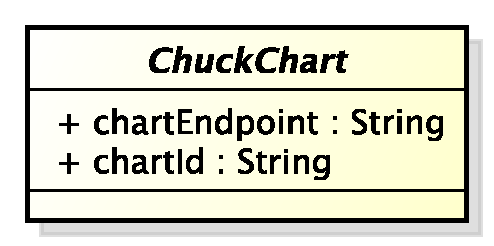
\includegraphics[scale=0.5]{DefinizioneDiProdotto/Pics/Classi/Chuck--Directive--ChuckChart}
				\caption{Chuck::Directive::ChuckChart}
			\end{figure}
		}
	
			
			\begin{itemize}
			\item \textbf{Nome:} ChuckChart
			\item \textbf{Tipo:} classe
			
		\item \textbf{Estende:}
		directive
		\item \textbf{Astratta:}
		si
			\item \textbf{Visibilità:} public
			\item \textbf{Descrizione:} Tale classe contiene le parti comuni necessarie per l'inserimento di un grafico.
			\item \textbf{Attributi:}
				\begin{itemize}
				\setlength{\itemsep}{5pt}
				
					\item[\ding{111}] {+chartEndpoint : String} \\ [1mm] Tale attributo permette di definire l'endpoint al quale è disponibile il grafico.
					\item[\ding{111}] {+chartId : String} \\ [1mm] Tale attributo permette di specificare l'id del grafico voluto.
				\end{itemize}
		
			\end{itemize}

			
			\level{5}[ChuckLineChart]{Chuck::Directive::ChuckLineChart}
			

		\IfFileExists{DefinizioneDiProdotto/Pics/Classi/Chuck--Directive--ChuckLineChart.pdf}{
			\begin{figure}[H]
				\centering
				\includegraphics[scale=0.5]{DefinizioneDiProdotto/Pics/Classi/Chuck--Directive--ChuckLineChart}
				\caption{Chuck::Directive::ChuckLineChart}
			\end{figure}
		}
	
			
			\begin{itemize}
			\item \textbf{Nome:} ChuckLineChart
			\item \textbf{Tipo:} classe
			
		\item \textbf{Estende:}
		ChuckChart
		\item \textbf{Astratta:}
		no
			\item \textbf{Visibilità:} public
			\item \textbf{Descrizione:} Tale classe permette di inserire un grafico di tipo LineChart all'interno di una pagina web.
			\item \textbf{Attributi:}
				\begin{itemize}
				\setlength{\itemsep}{5pt}
				
					\item[\ding{111}] {+datasetsColor : Color[]} \\ [1mm] Tale attributo permette di ridefinire i colori delle serie del chart.  Il tipo di tale attributo è un array di colori nel quale ogni oggetto rappresenta il colore della serie con il medesimo indice di posizionamento.
					\item[\ding{111}] {+legendPosition : String} \\ [1mm] Tale attributo permette di ridefinire la posizione della legenda.
					\item[\ding{111}] {+showGrid : boolean} \\ [1mm] Tale attributo permette di ridefinire se visualizzare la griglia o meno.
				\end{itemize}
		
			\end{itemize}

			
			\level{5}[ChuckMapChart]{Chuck::Directive::ChuckMapChart}
			

		\IfFileExists{DefinizioneDiProdotto/Pics/Classi/Chuck--Directive--ChuckMapChart.pdf}{
			\begin{figure}[H]
				\centering
				\includegraphics[scale=0.5]{DefinizioneDiProdotto/Pics/Classi/Chuck--Directive--ChuckMapChart}
				\caption{Chuck::Directive::ChuckMapChart}
			\end{figure}
		}
	
			
			\begin{itemize}
			\item \textbf{Nome:} ChuckMapChart
			\item \textbf{Tipo:} classe
			
		\item \textbf{Estende:}
		ChuckChart
		\item \textbf{Astratta:}
		no
			\item \textbf{Visibilità:} public
			\item \textbf{Descrizione:} Tale classe permette di inserire un grafico di tipo MapChart all'interno di una pagina web.
			\item \textbf{Attributi:}
				\begin{itemize}
				\setlength{\itemsep}{5pt}
				
					\item[\ding{111}] {+datasetsColor : Color[]} \\ [1mm] Tale attributo permette di ridefinire i colori delle serie del chart.  Il tipo di tale attributo è un array di colori nel quale ogni oggetto rappresenta il colore della serie con il medesimo indice di posizionamento.
					\item[\ding{111}] {+legendPosition : String} \\ [1mm] Tale attributo permette di ridefinire la posizione della legenda.
				\end{itemize}
		
			\end{itemize}

			
			\level{5}[ChuckTable]{Chuck::Directive::ChuckTable}
			

		\IfFileExists{DefinizioneDiProdotto/Pics/Classi/Chuck--Directive--ChuckTable.pdf}{
			\begin{figure}[H]
				\centering
				\includegraphics[scale=0.5]{DefinizioneDiProdotto/Pics/Classi/Chuck--Directive--ChuckTable}
				\caption{Chuck::Directive::ChuckTable}
			\end{figure}
		}
	
			
			\begin{itemize}
			\item \textbf{Nome:} ChuckTable
			\item \textbf{Tipo:} classe
			
		\item \textbf{Estende:}
		ChuckChart
		\item \textbf{Astratta:}
		no
			\item \textbf{Visibilità:} public
			\item \textbf{Descrizione:} Tale classe permette di inserire un grafico di tipo Table all'interno di una pagina web.
			\item \textbf{Attributi:}
				\begin{itemize}
				\setlength{\itemsep}{5pt}
				
					\item[\ding{111}] {+textColor : Color[][]} \\ [1mm] Tale attributo permette di ridefinire il colore del testo nelle celle della tabella. Il tipo di tale attributo è una matrice di colori perchè ogni cella rappresenta il colore del testo della cella della tabella nella medesima posizione.
					\item[\ding{111}] {+bgColor : Color[][]} \\ [1mm] Tale attributo permette di ridefinire il colore di sfondo nelle celle della tabella. Il tipo di tale attributo è una matrice di colori perchè ogni cella rappresenta il colore dello sfondo della cella della tabella nella medesima posizione.
				\end{itemize}
		
			\end{itemize}

			